\apendice{Plan de Proyecto Software}

\section{Introducción}

Para todo proyecto que se va a producir, es fundamental realizar un estudio acerca de cuales son los los objetivos que se quieren alcanzar, una planificación temporal y los recursos disponibles.
En este apartado se va a tratar sobre este establecimiento de metas y la temporalización de las mismas utilizando dos apartados principales:
\begin{itemize}
    \item Planificación temporal
    \item Estudio de viabilidad
    \begin{itemize}
        \item Viabilidad legal
        \item Viabilidad económica

    \end{itemize}

\end{itemize}


Debido a que se han utilizado metodologías ágiles durante el desarrollo de este proyecto, desde un inicio ha quedado muy claro cómo se gestionaban las tareas a realizar para poder ir generando un aporte de valor continuo tal como se muestra en la sección de planificación temporal.

Por otra parte, en el estudio de viabilidad se van a comentar tanto los aspectos económicos que conciernen al buen desarrollo del proyecto como el marco legal para tener garantizado que en un futuro no aparezcan inconvenientes legales

\section{Planificación temporal}
La planificación temporal del proyecto se ha estructurado en \textit{sprints} de aproximadamente dos semanas. Esta metodología ágil permite dividir el trabajo en ciclos cortos y manejables, facilitando la adaptación a los cambios y la mejora continua del desarrollo. Cada sprint incluye la planificación, ejecución y revisión de un conjunto de tareas específicas, asegurando que el proyecto avance de manera constante y controlada.

\subsection{Primer \textit{sprint} 29-11-2023 / 20-12-2023}
Antes de la selección de herramientas y tecnologías, se llevaron a cabo una serie de reuniones con el cliente para capturar y entender los requisitos del proyecto. Estas reuniones son cruciales para asegurar que todas las necesidades y expectativas del cliente se consideren desde el principio.
Como primeros pasos para la creación del proyecto, se realiza un estudio inicial para considerar cuales van a ser los lenguajes de programación utilizados durante el proyecto. Debido a mi poca experiencia diseño web, opto por utilizar el \textit{framework} de python \href{https://flask.palletsprojects.com/en/3.0.x/}{Flask} ya que de una manera sencilla me permite crear páginas web en un lenguaje de programación ya trabajado durante la carrera y tener una integración sencilla entre \textit{backend} y \textit{frontend}. Además de esta elección, en esta tarea se realizan labores de investigación y lectura de documentación para iniciar el proyecto con las habilidades suficientes para empezar a dar pequeños pasos en el diseño web.
Algún ejemplo de la documentación utilizada es la página oficial de Flask~\cite{Flask} y la documentación de Bootstrap5~\cite{Bootstrap5}.

Como otra tarea a realizar durante este sprint, se determina como idea inicial obtener los datos de los libros a través de la realización de peticiones a una API . Esto permitía una manera simple de obtener unos datos alojados en internet y poder generar un filtro  para obtener el resultado esperado.
Tal como se menciona en la memoria, se inclina la balanza a favor de la API de Google, por lo que inicio la lectura de documentación asociada para informarme sobre cómo realizar las llamadas a este servicio.

Mientras se realizan esas tareas se toman apuntes para incluir la información de la API en la memoria.

Tras definir las tareas a realizar en este \textit{sprint}, se estimó que la duración de la realización de las tareas son de 10 horas, pero finalmente las tareas se completan en 7 horas.

\subsection{Segundo \textit{sprint} 20-12-2023 / 16-01-2024}

Tras tomar las decisiones iniciales del anterior \textit{sprint}, comienzo a investigar la estructura del Framework y los lenguajes HTML y CSS realizando pequeños ejercicios , ya que mi experiencia anterior con estas herramientas era muy limitada.

Una vez realizada esa toma de contacto  creo una ejemplo inicial de como podría estructurarse la web para debatirlo en la reunión de fin de \textit{sprint}.
Para este inicialmente creo un catálogo básico  con una base de datos que permite realizar estas operaciones de manera manual:

\begin{itemize}
    \item Barra de navegación que permite cambiar de página.
    \item Sistema de Login para gestionar la aparición de botones ocultos.
    \item Consultar todos los libros existentes en la base datos.
    \item Realizar búsquedas de los libros existentes en la base de datos en base al título o al ISBN.
    \item Agregar un libro a la base de datos.
    \item Editar un libro de la base de datos.
    \item Eliminar un libro de la base de datos.

\end{itemize}

El sistema de Login se estableció para no permitir que ningún usuario que no tuviese credenciales pudiera realizar modificaciones de la base de datos. En el caso de que ejecutaran la URL exacta de la función, la protección de seguridad les llevaría a la pantalla de Inicio de Sesión.

\begin{figure}[h]
    \centering
    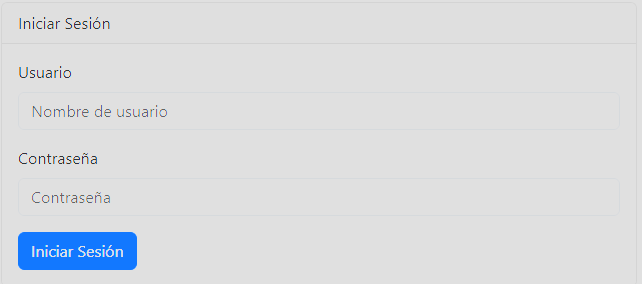
\includegraphics[width=0.9\textwidth]{Imagenes/Inicio_Sesion.png}
    \caption{Inicio de sesión}
    \label{Inicio de sesión}
\end{figure}

Para poder tener más libertad de elementos para integrar dentro de la web, se decide utilizar la biblioteca Bootstrap 5, la cual tiene elementos predefinidos con estilos, generando una programación más eficiente y limpia.

Mientras continuo realizando apuntes para incluirlos en la memoria posteriormente.

Realizar estas tareas tuvo una estimación inicial de 45 horas, pero finalmente fueron 40 horas.

\subsection{Tercer \textit{sprint} 16-01-2024 / 30-01-2024}

Una vez presentado y debatido este primer prototipo de página web en el \textit{sprint}, se decide continuar de esta base agregando más elementos para añadirle funcionalidades. De manera adicional, se comienza a realizar un prototipo web para ir documentando el esquema de secciones existente en este proyecto. Tal como se comenta en la sección de Técnicas y Herramientas,  el prototipo web se realiza con el programa Justinmind.

Además, se agrega otra funcionalidad considerada como esencial, una página que al seleccionar el libro te muestre toda la información disponible en la base de datos para todo usuario interesado en obtener datos.
Para ello, en cada libro mostrado en el catálogo se pone a disposición un botón que te redirige a esta página.

Durante esa reunión se propone la idea de incluir un apartado especifico para los responsables de la administración que permite importar y exportar en un archivo CSV todos los datos de cada libro contenidos en la base de datos. 
Esta idea se concibe principalmente por dos grandes motivos
\begin{itemize}
    \item Tener la oportunidad de volcar datos más rápido desde el archivo CSV y posteriormente cargar el contenido del fichero en la base de datos.
    \item Poder tener un duplicado de la base de datos por si el contenido de la misma quedase inaccesible o se realizara un cambio indeseado, lo cuál se solucionaría restableciendo el catálogo con el archivo de seguridad descargado.
\end{itemize}

Realizar estas tareas tuvo una estimación inicial de 40 horas, pero finalmente fueron 36     horas.

\subsection{Cuarto \textit{sprint} 30-1-2024 / 13-02-2024}
En este \textit{sprint} se corrigieron un error relativo a la implementación de la importación y la exportación
El error consistía en que un administrador pudiera colocar el signo "," para separar dos elementos como por ejemplo dos ISBN o que se encontrase en el contenido de la descripción del libro, lo cual generaba errores a la hora de transformar los campos a columnas al tener ese mismo signo como delimitador. Por ese motivo se propuso la idea de cambiar el delimitador por defecto a el signo ";".

Tras realizar estas correcciones de errores iniciamos el proceso de obtener la información  de los libros de forma automática. Aunque inicialmente se valoró la opción de utilizar únicamente la API de Google Books,  se consideró interesante para  dar más fuentes de información y aumentar la dificultad técnica del proyecto la utilización de Web scraping. 
El  web scraping realizado se aplica sobre 2 páginas web las cuales tienen un catálogo de libros muy amplio. Estas webs son \href{https://www.amazon.es/}{Amazon} y \href{https://www.agapea.com/}{Agapea}. Estos tres proveedores nos permiten que en base a un ISBN o un Título, internamente se lancen unos procesos que busquen en los proveedores con las diferentes técnicas mostradas para que se pueda seleccionar el proveedor que nos de la información más precisa. 
En el caso de que se quisiera agregar un libro automáticamente pero se desee personalizar y usar una mezcla de los 3 proveedores, se dispone de un sistema de desplegables que nos permite realizar esta acción.

Durante el desarrollo en este espacio de tiempo, se considera que sería necesario implementar un sistema que nos permitiese proteger el catálogo de una importación que pueda encontrarse corrupta o con datos erróneos.
Por lo que antes de realizar la importación, aparece una ventana modal que recuerda al usuario que debería de exportar el catálogo actual por seguridad.

Para este \textit{sprint} se estimo inicialmente unas 30 horas pero finalmente se realizó en 35.

\subsection{Quinto \textit{sprint} 13-02-2024 / 27-02-2024}
Tras hacer las pruebas pertinentes de que la técnica de Web scraping es satisfactoria en y una gran mayoría de casos devuelve el libro correcto, (Los casos en los que falla es debido a la inexistencia de ese título en el catálogo de la plataforma en la que se busca), se pone como tareas en este \textit{sprint} integrarlo a la página web en un apartado específico de búsqueda automática y acompañarlo de la llamada a la API de Google books. Para indicar al usuario que se esta ejecutando la búsqueda de libros, se añade una animación de carga.

Finalmente se pone como tarea el tratamiento de los datos obtenidos de esas fuentes, indicando con botones cual de los resultados de las fuentes es el deseado para agregar al catálogo.
En el caso de que se quisiera agregar un libro automáticamente pero se desee personalizar y usar una mezcla de los 3 proveedores, se dispone de un sistema de desplegables que nos permite realizar esta acción.

Durante el desarrollo en este espacio de tiempo, se considera que sería necesario implementar un sistema que nos permitiese proteger el catálogo de una importación que pueda encontrarse corrupta o con datos erróneos.
Por lo que antes de realizar la importación, aparece una ventana modal que recuerda al usuario que debería de exportar el catálogo actual por seguridad.

Este \textit{sprint} recibió una estimación inicial de 30 horas pero se completaron todas las tareas en 20 horas.

\subsection{Sexto \textit{sprint} 27-02-2024 / 2-04-2024}
En la reunión de inicio de este \textit{sprint} se presentó la idea acerca de la posibilidad de cambiar la parte de \textit{frontend} hasta ahora implementada utilizando Flask a un framework más potente llamado Angular. Esto se debe a que durante mis prácticas curriculares obtuve conocimientos de este framework, que además de utilizar HTML y CSS utiliza TypeScript para el desarrollo de las aplicaciones.
Tras hablarlo decidimos que este \textit{sprint} se dedicaría a investigar la viabilidad de una refactorización completa del \textit{frontend} a Angular mientras se realizaban desarrollos en la aplicación ya creada. 
De manera adicional, para poder realizar un intercambio de información óptima el \textit{backend} de Flask tendría que modificarse para convertirse en una API. Por lo que se realizó este estudio también.

Como desarrollo en paralelo en la aplicación actual se propuso generar un formulario de ejemplo acerca de la predicción de valoración de un libro.

El tiempo estimado inicial es de 20 horas pero las tareas se completan finalmente en 30 horas.

\subsection{Séptimo \textit{sprint} 13-03-2024 / 2-04-2024}
Durante este \textit{sprint} se definieron las tareas a refactorizar al nuevo framework, después de un resultado positivo en la investigación de viabilidad, por lo que numerosas pantallas generadas en flask se refactorizaron y modificaron para adaptarla al nuevo framework. 
Como tarea adicional, se definió nuevas pantallas que permitían tener un entorno de usuario más limpio y clasificado para todos los usuarios de la web. Un ejemplo de esto es la creación de un panel de administración.
Para poder agregar aún más elementos y variedad a la web, se incluyeron las siguientes bibliotecas que brindan un catálogo de elementos extenso:
\begin{itemize}
    \item PrimeNG
    \item Sweetalert2
\end{itemize}

Por la parte del \textit{backend}, se modificaron todos los métodos para poder utilizarse como API y trabajar con archivos de formato JSON. Esto permite tener separado el \textit{frontend} y el \textit{backend}.

Estas tareas tuvieron una estimación de 80 horas y se completaron en 100 horas


\subsection{Octavo \textit{sprint} 2-04-2024 / 16 -4-2024}
Durante este \textit{sprint} se completaron de refactorizar los apartados no contemplados en el \textit{sprint} anterior y se decidió mejorar la personalización de la página web para que los responsables de la administración de la misma tuvieran el mayor control posible y aumentar la complegidad técnica de la web.
Algunas de estas decisiones fueron implementar un sistema de usuarios personalizados con un sistema de roles totalmente gráficos, y cada uno de esos roles contiene una serie de permisos personalizables y ajustables, limitando de manera dinámica a los usuarios con cuenta ciertos parámetros del panel de administrador.

Otra tarea perteneciente a este \textit{sprint} consiste en aplicar esa misma filosofía de personalización, permitiendo tanto guardar las estimaciones realizadas por los usuarios como modificar ciertos parámetros de elección en ese apartado de estimaciones.

Finalmente, por agregar funcionalidades distintas se creó una tarea de creación de un apartado de sugerencias las cuales mandarían el contenido de esa sugerencia automáticamente a una cuenta de correo expresamente creada para ese fin.

Este \textit{sprint} ha tenido una estimación inicial de 50 horas y se dedicaron 70.

\subsection{Noveno \textit{sprint} 16-04-2024 / 30-04-2024}
En este \textit{sprint} se propone ir cerrando todas las tareas de desarrollo restantes para poder desplegar la aplicación completa y comenzar con el testing.
Se han definido tareas como un apartado de estadísticas para dar una visión a los usuarios con cuenta de las estadísticas actuales de los libros y de otros parámetros.
Estas tareas engloban tanto el desarrollo del \textit{backend} como la implementación de los resultados en el \textit{frontend}.

De manera adicional, se van corrigiendo errores de la página para que sea completamente adaptativa al tamaño de la pantalla, así como errores de importación y exportación de CSV y la inclusión del formato Excel.

Finalmente, también se crean unos ejemplos de como sería el formato de las páginas pendientes de rellenar.

Este \textit{sprint} ha tenido una estimación inicial de 20 horas, y se finalizó en un tiempo de 15 horas.


\subsection{Décimo \textit{sprint} 30-04-2024 / 14-05-2024}
En este \textit{sprint} se realiza el despliegue tanto en netlify como en render para front y back respectivamente, con esto ya se pueden realizar pruebas más estrictas para terminar de perfilar los detalles y comenzar a localizar errores.

Además de eso, se comienza a separar todos los archivos del \textit{backend} en módulos para facilitar la independencia, mantenibilidad y escalabilidad.

De manera adicional, se van corrigiendo errores del apartado responsive para que se pueda ver la web correctamente en dispositivos móviles y se integra JWT para evitar llamadas a la API de usuarios no autorizados.

Este \textit{sprint} ha tenido un estimación inicial de 50 horas y finalmente se dedicaron 60 debido a problemas en el despliegue.

\subsection{Undécimo \textit{sprint} 14-05-2024 / 28-04-2024}
Este \textit{sprint} se dedica íntegramente a realizar la memoria e ir localizando errores que se van localizando. 
Un error muy significativo encontrado al desplegar ha sido la persistencia de los datos en la base de datos, por lo que se decidió pagar la suscripción mínima para poder tener esa persistencia y poder realizar pruebas con base de datos.

Otro de los errores importantes tratados durante este \textit{sprint} ha sido el apartado de estadísticas, el cual si se importaban libros fallaba la generación de estadísticas y no se tenían en cuenta los libros ya existentes en el catálogo antes de realizar la importación.

La estimación de este apartado ha sido de 70 horas pero se pudo completar en 50 horas.

\subsection{Duodécimo \textit{sprint} 28-04-2024 / 4-04-2024}
Durante la realización de este \textit{sprint}, se realizó una reunión para evaluar la viabilidad de realizar nuevos desarrollos y cambios menores, los cuales se revisaron, se adaptaron y se aceptaron. 

Uno de esos cambios es la realización de un nuevo apartado en la web que describa la intencionalidad de la página web y muestre una tabla con todos los colaboradores que han realizado aportaciones verídicas e interesantes en el apartado de valoración, los cuales sirven de guía para los responsables de la administración para poder generar una valoración más profunda.

Por otra parte, se continúa con el desarrollo de la memoria y los anexos y se sigue continuando con las pruebas de la página web, intentando localizar más errores o cambios mínimos como el idioma del calendario del selector de rango de las estadísticas.

Este \textit{sprint} tiene una valoración temporal de 30 horas pero se han dedicando 45 horas.


\subsection{Resumen de horas estimadas y dedicadas}
Se puede observar en la gráfica inferior un resumen visual de las horas estimadas junto con las horas realizadas. Si se analiza este gráfico, se puede concluir que las horas estimadas y las horas dedicadas a la realización del proyecto siempre han tenido una relación aproximada (sin grandes variaciones), por lo que aún apareciendo problemas y soluciones más eficientes a lo largo de los \textit{sprints}, todos han tenido una estimación relativamente cercana al esfuerzo real que se ha llevado a cabo.

\begin{figure}[h]
    \centering
    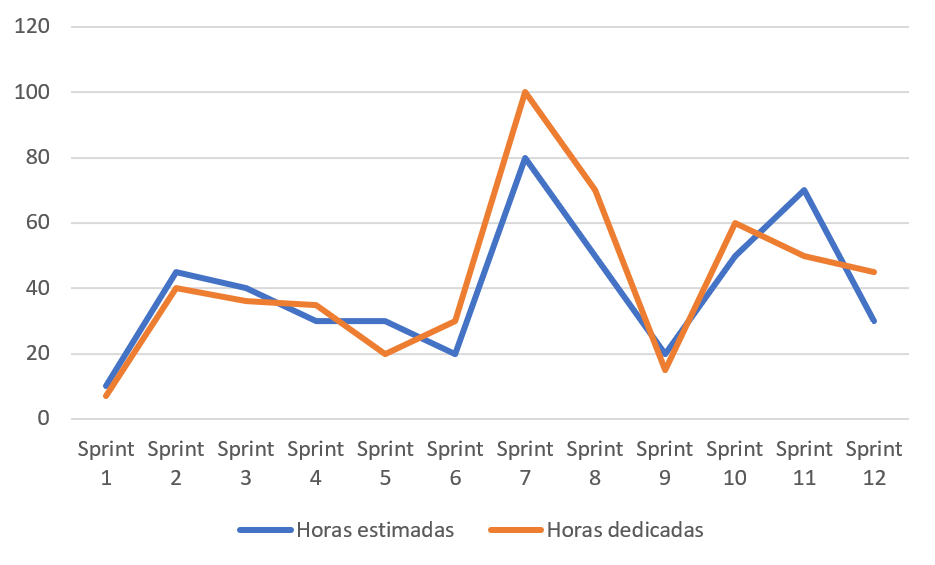
\includegraphics[width=1\linewidth]{Imagenes/GraficoSprint.png}
    \caption{Gráfico de horas de sprints}
    \label{Gráfico de horas de sprints}
\end{figure}
\FloatBarrier

\section{Estudio de viabilidad}
Dentro de este apartado se analiza la viabilidad del proyecto desde varios puntos de vista: la viabilidad económica y la viabilidad legal. A continuación se explica más detalladamente cada uno de los subapartados.

\subsection{Viabilidad económica}
La viabilidad económica es un aspecto fundamental en todo proyecto software debido a que estudia tanto los costes como los beneficios que van a producirse a lo largo del desarrollo.

El análisis de costes y beneficios se ha realizado suponiendo que el proyecto se ha llevado a cabo en un entorno empresarial real en el ámbito español. Esto incluye la consideración de los salarios, impuestos y contribuciones a la seguridad social según la normativa vigente.

\subsubsection*{Costes de Personal}
Teniendo en cuenta que se han dedicado 472 horas en total para el desarrollo del proyecto y que el salario bruto medio en Castilla y León es 21773€\footnote{Bankinter: \url{https://www.bankinter.com/blog/mercados/salario-medio-espana-comparativa}}, el salario bruto correspondiente a ese tiempo es de 2950€


\begin{tabular}{lrr}
\toprule
Descripción & Coste Bruto \\
\midrule
Sueldo Bruto & 2,950€ \\
IRPF (11,64\%) & -344€ \\
\textbf{Sueldo Neto} & \textbf{2,606€} \\
\bottomrule
\end{tabular}

Tal como se puede observar, se ha realizado un cálculo simulado incluyendo la retención del IRPF, se obtiene un valor final de 2,606 euros netos de salario.

\subsubsection*{Costes de Hardware}

\begin{tabular}{lrr}
\toprule
Descripción & Coste Total & Amortización Anual \\
\midrule
Ordenador de desarrollo & 1,000€ & 200€ \\
Periféricos (monitor, teclado, ratón) & 300€ & 60€ \\
\textbf{Total} & \textbf{1,300€} & \textbf{260€} \\
\bottomrule
\end{tabular}

En este apartado tenemos en cuenta el valor del hardware que se ha utilizado, tanto el ordenador como sus periféricos. Para que los cálculos se correspondan con la realidad, se realiza una amortización a 5 años de los elementos utilizados.

\subsubsection*{Costes de Software}

\begin{tabular}{lrr}
\toprule
Descripción & Coste Total & Amortización Anual \\
\midrule
Licencia de Sistema Operativo (Windows 10 Pro) & 200€ & 40€ \\
Servidor de Render (pago anual) & 84€ & 84€ \\
\textbf{Total} & \textbf{284€} & \textbf{124€} \\
\bottomrule
\end{tabular}

Los costes de software son reducidos ya que se ha trabajado lo máximo posible con bibliotecas y sofware gratuito que no necesita recibir ningún tipo de pago, exceptuando el host del \textit{backend} por motivos de persistencia de datos
Debido al motivo expuesto, solo se tiene en cuenta el sistema operativo del ordenador utilizado con una amortización similar a los elementos de hardware (Duración de 5 años), y el servicio de host de pago mensual y con un valor anual mostrado en la tabla.

\subsubsection*{Costes Varios}

\begin{tabular}{lr}
\toprule
Descripción & Coste Anual \\
\midrule
Internet y comunicaciones & 600€ \\
Electricidad y otros suministros de oficina & 300€ \\
 Coste curso formación angular&200€\\
\textbf{Total} & \textbf{1100€}\\
\bottomrule
\end{tabular}

Estos costes van referidos a todos aquellos externos al sistema en el que se desarrolla el proyecto pero son esenciales para una correcta continuidad y trabajo. 
Actualmente de este apartado solo ha sido necesario tener en cuenta servicios como internet y electricidad ya que no se han usado elementos físicos extra para el desarrollo.
De manera adicional, para la creación de este proyecto también se ha tenido en cuenta el coste de los cursos realizados.
\subsubsection*{Total de Costes Directos}

\begin{tabular}{lr}
\toprule
Descripción & Coste \\
\midrule
Personal (Neto) & 2,606€ \\
Hardware (Amortización) & 260€ \\
Software (Amortización) & 124€\\
Varios & 1100€\\
\textbf{Total Anual} & \textbf{4,090€}\\
\bottomrule
\end{tabular}

Esta tabla muestra un resumen de la suma de los gastos anuales de todos los apartados anteriormente mencionados, por lo que anualmente este proyecto cuesta realizarle 4,090 euros.

\subsubsection{Beneficios}
Este proyecto no ha tenido en cuenta una retribución por el uso o distribución del programa ya que su objetivo es ser una fuente fiable de información y gratuita para todos las personas usuarias, y especialmente enfocado a fines didácticos y sociales.
\subsection{Viabilidad legal}
Para poder analizar la viabilidad legal de este proyecto es inicialmente necesario comprobar todas las bibliotecas externas utilizadas en las funcionalidades.
En la tabla de debajo se listan las dependencias principales con sus respectivas licencias, las cuales nos pueden llegar a limitar los permisos y las restricciones que podemos implantar en los usuarios.

\begin{table}[ht]
\centering
\begin{tabular}{@{}lll@{}}
\toprule
Biblioteca & Descripción & Licencia \\ 
\midrule
Flask & Microframework web para Python & BSD \\
Flask-Bcrypt & Proporciona utilidades Bcrypt para Flask & MIT \\
Flask-Cors & Manejo de CORS en aplicaciones Flask & MIT \\
Flask-JWT-Extended & Extensiones JWT para Flask & MIT \\
Flask-Login & Manejo de sesiones de usuario en Flask & MIT \\
Flask-RESTful & Extensión para construir APIs en Flask & BSD \\
Flask-SQLAlchemy & Extensión de Flask para SQLAlchemy & MIT \\
SQLAlchemy & Toolkit SQL y ORM para Python & MIT \\
openpyxl & Librería para leer/escribir archivos Excel & MIT \\
requests & Librería para realizar peticiones HTTP & Apache License 2.0 \\
gunicorn & Servidor HTTP WSGI para UNIX & MIT \\
beautifulsoup4 & Librería para parsear documentos HTML & MIT \\
PrimeNG & Librería para elementos Angular & MIT \\
SweetAlert2 & Librería para modales & MIT \\
\bottomrule
\end{tabular}
\caption{Resumen de licencias de las bibliotecas utilizadas en el proyecto}
\end{table}
\FloatBarrier
Una vez obtenidas las licencias, las ordenamos de más restrictivas a menos:
\begin{itemize}
\begin{enumerate}
    \item Apache License 2.0
    \begin{itemize}
        \item Descripción: Esta licencia de software libre y de código abierto es menos restrictiva que la GPL y permite a los usuarios del software la libertad de usar, modificar, y distribuir el software como lo vean conveniente, siempre que se incluyan las notas de derechos de autor y las licencias de todas las copias o versiones sustanciales del software.~\cite{apache_license}
        \item Ejemplo de biblioteca: \verb|requests|
    \end{itemize}
    \item MIT License
    \begin{itemize}
        \item Descripción: La licencia MIT es una de las licencias de software más permisivas. Permite el uso, copia, modificación, fusión, publicación, distribución, sublicencia, y/o venta de copias del software, sin restricciones siempre que se mantenga el aviso de derechos de autor original.\cite{mit_license}
        \item Ejemplos de bibliotecas: \verb|Flask-Bcrypt|, \verb|Flask-Cors|, \verb|Flask-JWT-Extended|, \verb|Flask-Login|, \verb|Flask-SQLAlchemy|, \verb|gunicorn|, \verb|openpyxl|
    \end{itemize}
    \item BSD License
    \begin{itemize}
        \item Descripción: Las licencias BSD son otra familia de licencias de software libre permisivas que tienen menos restricciones comparadas con Apache, permitiendo el uso y redistribución del software con o sin modificación. No se requiere la redistribución del código fuente.\cite{bsd_license}
        \item Ejemplos de bibliotecas: \verb|Flask|, \verb|Flask-RESTful|
    \end{itemize}
\end{enumerate}
 
\end{itemize}

Teniendo en cuenta toda esta información, la decisión más acertada para este proyecto sería una licencia de \textbf{MIT}. Esto se debe a que es una licencia simple que permite a las personas usuarias realizar operaciones y modificaciones por cuenta propia al programa siempre que se incluya el aviso de derechos de autor.
Esto permitiría que más allá de las competencias del cliente en cuestión se pueda desarrollar y adaptar para otras necesidades educativas.

En cuanto a la documentación y las imágenes, todo lo incluido de terceros cuenta con Creative Commons. 
Como el programa en sí tiene una licencia que permite modificaciones, la elección es \textbf{Creative Commons}, concretamente la licencia \textbf{CC BY}, la cuál permite su uso siempre que se de crédito al autor original.~\cite{cc_by_license}

\begin{table}[ht]
    \centering
    \begin{tabular}{cc}
        \toprule
         Elemento & Licencia\\
         \midrule
         Código fuente & MIT\\
         Documentación & CC BY\\
         Imágenes & CC BY \\
         \bottomrule
    \end{tabular}
    \caption{Resumen de licencias utilizadas}
\end{table}